% UN PREMIER DOCUMENT !!
\documentclass[a4paper, twoside]{article}

% PACKAGES / LIBRAIRIES
\usepackage[utf8]{inputenc} % Definition de l'encodage du fichier .tex
\usepackage[bitstream-charter]{mathdesign} % CHARTER BT FONT
%\usepackage[condensed,math]{iwona}
\usepackage[T1]{fontenc}
\usepackage[francais]{babel} % normes typographiques spécifiques à une langue.
\usepackage{amsmath, amsfonts} % amélioration de l'affichage et de la définition des fonctions mathématiques
\usepackage{graphicx} % Insertion de figures avec \includegraphics[scale=•]{•}
\usepackage{blindtext} % Texte aléatoire pour meubler le document
\blindmathtrue
\usepackage{authblk} % Authors and affiliations

% SETUP DU DOCUMENT
\title{Mon premier document avec \LaTeX} % Définition du titre
%\author{L. Charleux\thanks{It's also me} \\ \url{mailto:ludch@univ-smb.fr} \and 
%        L. Charleux \\ \url{mailto:ludch@univ-smb.fr}}
\author[,1]{Mark Knopfler\thanks{Corresponding author: \texttt{haggis\_power@wanadoo.fr}}}
\author[2,3]{Jimmy Page}
\author[,2]{Ian Gillan\thanks{Now at: elsewhere}}
\author[,3]{David Gilmour\thanks{Now at: elsewhere}}
 
\affil[1]{University of Glasgow, Scotland, United Kingdom}
\affil[2]{Imperial College London, London, England, United Kingdom}
\affil[3]{University of Cambridge, England, United Kingdom}

\date{Mardi 2 juin 2020}
\usepackage[left = 5cm,  % Marge intérieure
            right = 1cm, % Marge extérieure (en twoside)
            top = 2cm,
            bottom = 2cm]{geometry}

%\setlength{\parskip}{1cm} % Espace entre paragraphes
\usepackage{hyperref}
\hypersetup{
    bookmarks=true,         % show bookmarks bar?
    unicode=false,          % non-Latin characters in Acrobat’s bookmarks
    pdftoolbar=true,        % show Acrobat’s toolbar?
    pdfmenubar=true,        % show Acrobat’s menu?
    pdffitwindow=false,     % window fit to page when opened
    pdfstartview={FitH},    % fits the width of the page to the window
    pdftitle={Mon premier document},    % title
    pdfauthor={Dora l'exploratrice},     % author
%    pdfsubject={Subject},   % subject of the document
%    pdfcreator={Creator},   % creator of the document
%    pdfproducer={Producer}, % producer of the document
%    pdfkeywords={keyword1, key2, key3}, % list of keywords
    pdfnewwindow=true,      % links in new PDF window
    colorlinks=false,       % false: boxed links; true: colored links
    linkcolor=red,          % color of internal links (change box color with linkbordercolor)
    citecolor=green,        % color of links to bibliography
    filecolor=magenta,      % color of file links
    urlcolor=cyan           % color of external links
 }

\usepackage[squaren,Gray]{SIunits} % Gestion des unités physiques

% DOCUMENT
\begin{document}
\maketitle % Affichage du titre


\begin{abstract}
Le bigorneau - mot probablement dérivé de \textbf{bigorne} dans l'acception usuelle et notamment commerciale, est le plus consommé des petits gastéropodes marins à coquille spiralée. Dans ce sens, il correspond à l'espèce Littorina littorea. Du fait de son importance économique, ce nom est compris et utilisé partout, y compris au Québec où il a fait l'objet d'une décision de normalisation par l'Office québécois de la langue française. Plus largement, la dénomination englobe les autres espèces du genre Littorina et par extension celles de la sous-famille des Littorininae, les \og littorines \fg. 
\end{abstract}

\tableofcontents % Table des matières

\section*{Introduction} % le "*" veut dire que la section n'est pas numérotée
\addcontentsline{toc}{section}{\protect\numberline{}Introduction} %On ajoute "Introduction" à la table des matières

La loutre de mer ne doit pas être confondue avec la \og loutre marine \fg, Lontra felina, encore appelée chat de mer ou chungungo, qui vit le long des côtes du Pérou et du Chili et qui a besoin d'abris terrestres. 
Il arrive aussi quelquefois que certaines loutres d'eau douce, comme la loutre d'Europe, fassent des incursions en mer (le cas est même assez fréquent dans certains pays comme en Irlande), mais leur organisme n'est pas adapté à des séjours prolongés. 

Chassées intensivement à compter de 1741 pour leur fourrure (la plus dense de tous les mammifères avec jusqu'à 170 000 poils par centimètre carré), les populations de loutre de mer ont été considérablement réduites, disparaissant même de nombreuses régions de leur zone de répartition historique. 
En 1911 on a estimé que leur population mondiale était tombée entre 1 000 et 2 000 individus. 
Bien que plusieurs sous-espèces soient encore en danger, les loutres marines, qui sont légalement protégées, ont vu leur population fortement augmenter. Les efforts de réintroduction ont également montré des résultats positifs.


\section{État de l'art}
\subsection{Un truc}

On considère une équation très profonde Eq. \ref{eq:math_simples} (voir page \pageref{eq:math_simples}):

$$ % Ouverture d'une équation
v(x) = \int_{0}^{+\infty} u(x) dx 
$$ % Fermeture d'une équation

\begin{align}
& u  =   5 \\
& v = 12
\end{align}

\begin{equation}
2+ 2 = 4
\label{eq:math_simples}
\end{equation}

\begin{equation}
f(x) = \left\lbrace 
\begin{split}
0 \mbox{ if } x \leq 0 \\
x^2 \mbox { otherwise}
\end{split}
\right.
\end{equation}


$$
I_3 = 
\begin{bmatrix}
1 & 0 & 0 \\
0 & 1 & 0 \\
0 & 0 & 1 
\end{bmatrix}
$$

$$
\alpha \xi \Xi \phi \Psi
$$

$$
a b c
$$

\subsection{Un autre trucs}



\section{Une section à part}

blabla \dots % On insère un autre document.

\section{Insertion de figures}
\label{sec:figures}

Je vois un panda ici 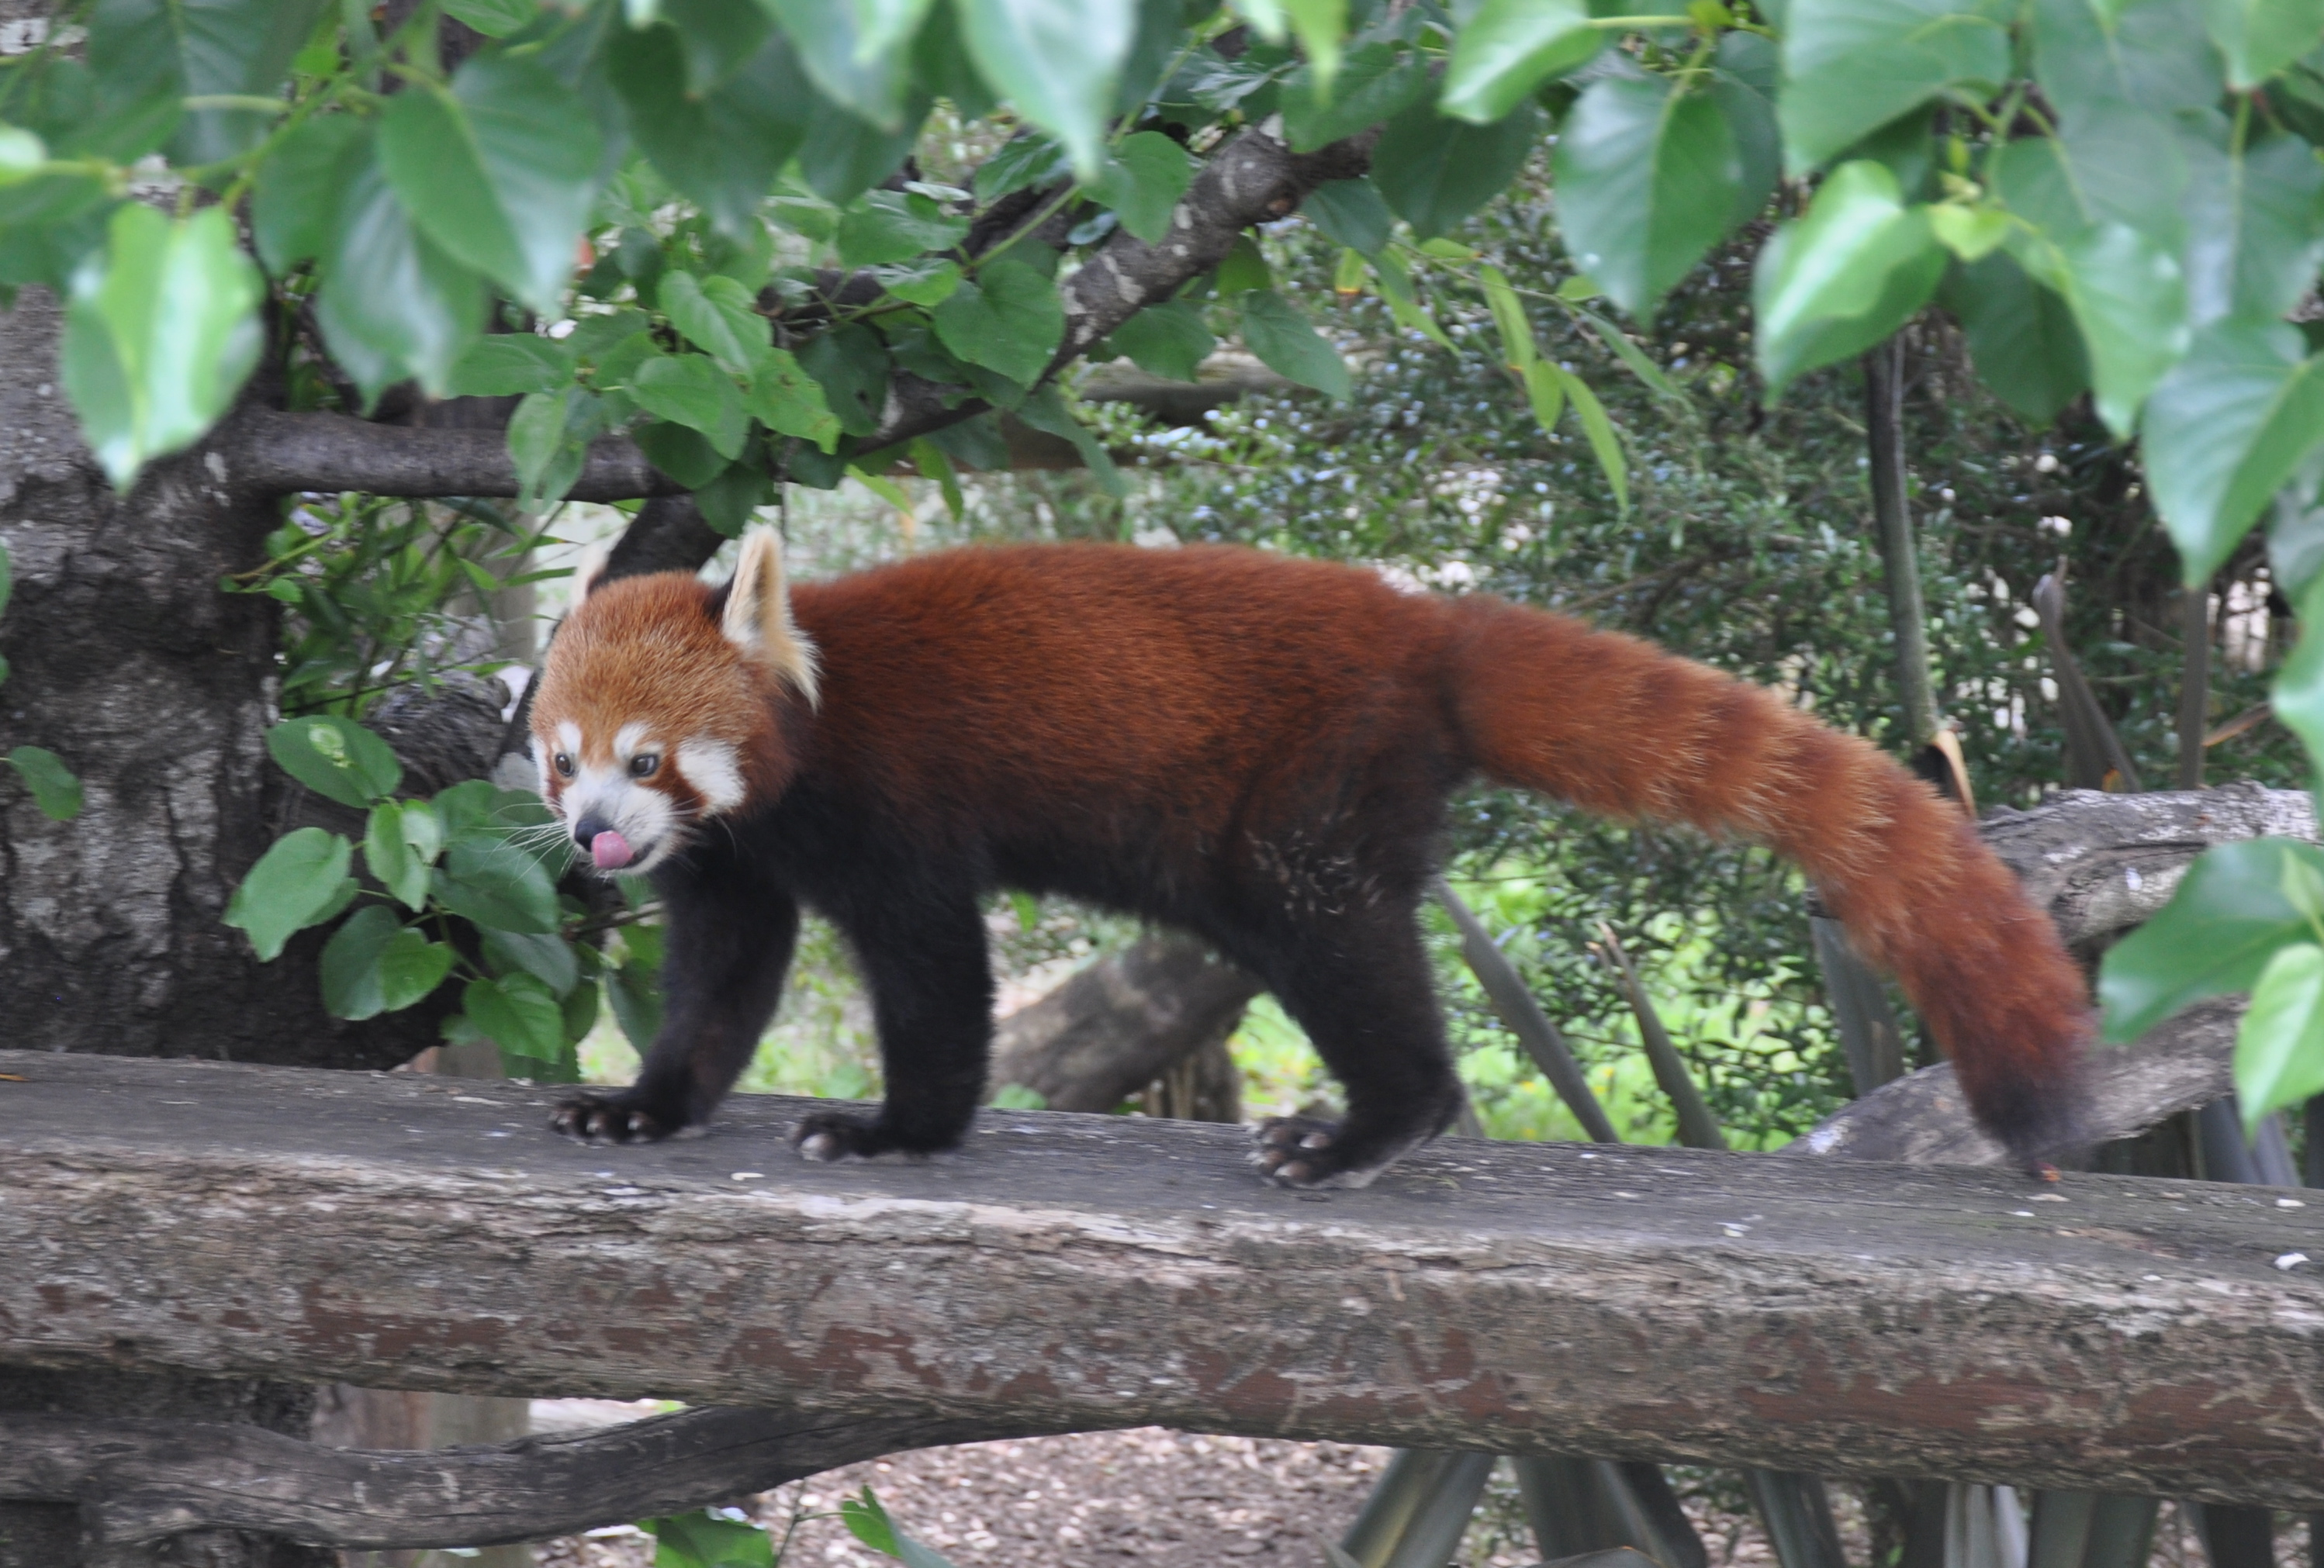
\includegraphics[scale=.01]{figures/panda.JPG} et là. En particulier, on le voit sur la figure Fig. \ref{fig:panda_roux} (page \pageref{fig:panda_roux}) dans la partie \ref{sec:figures}.

%\blindmathpaper[5]

\begin{figure}[h]
\begin{center}
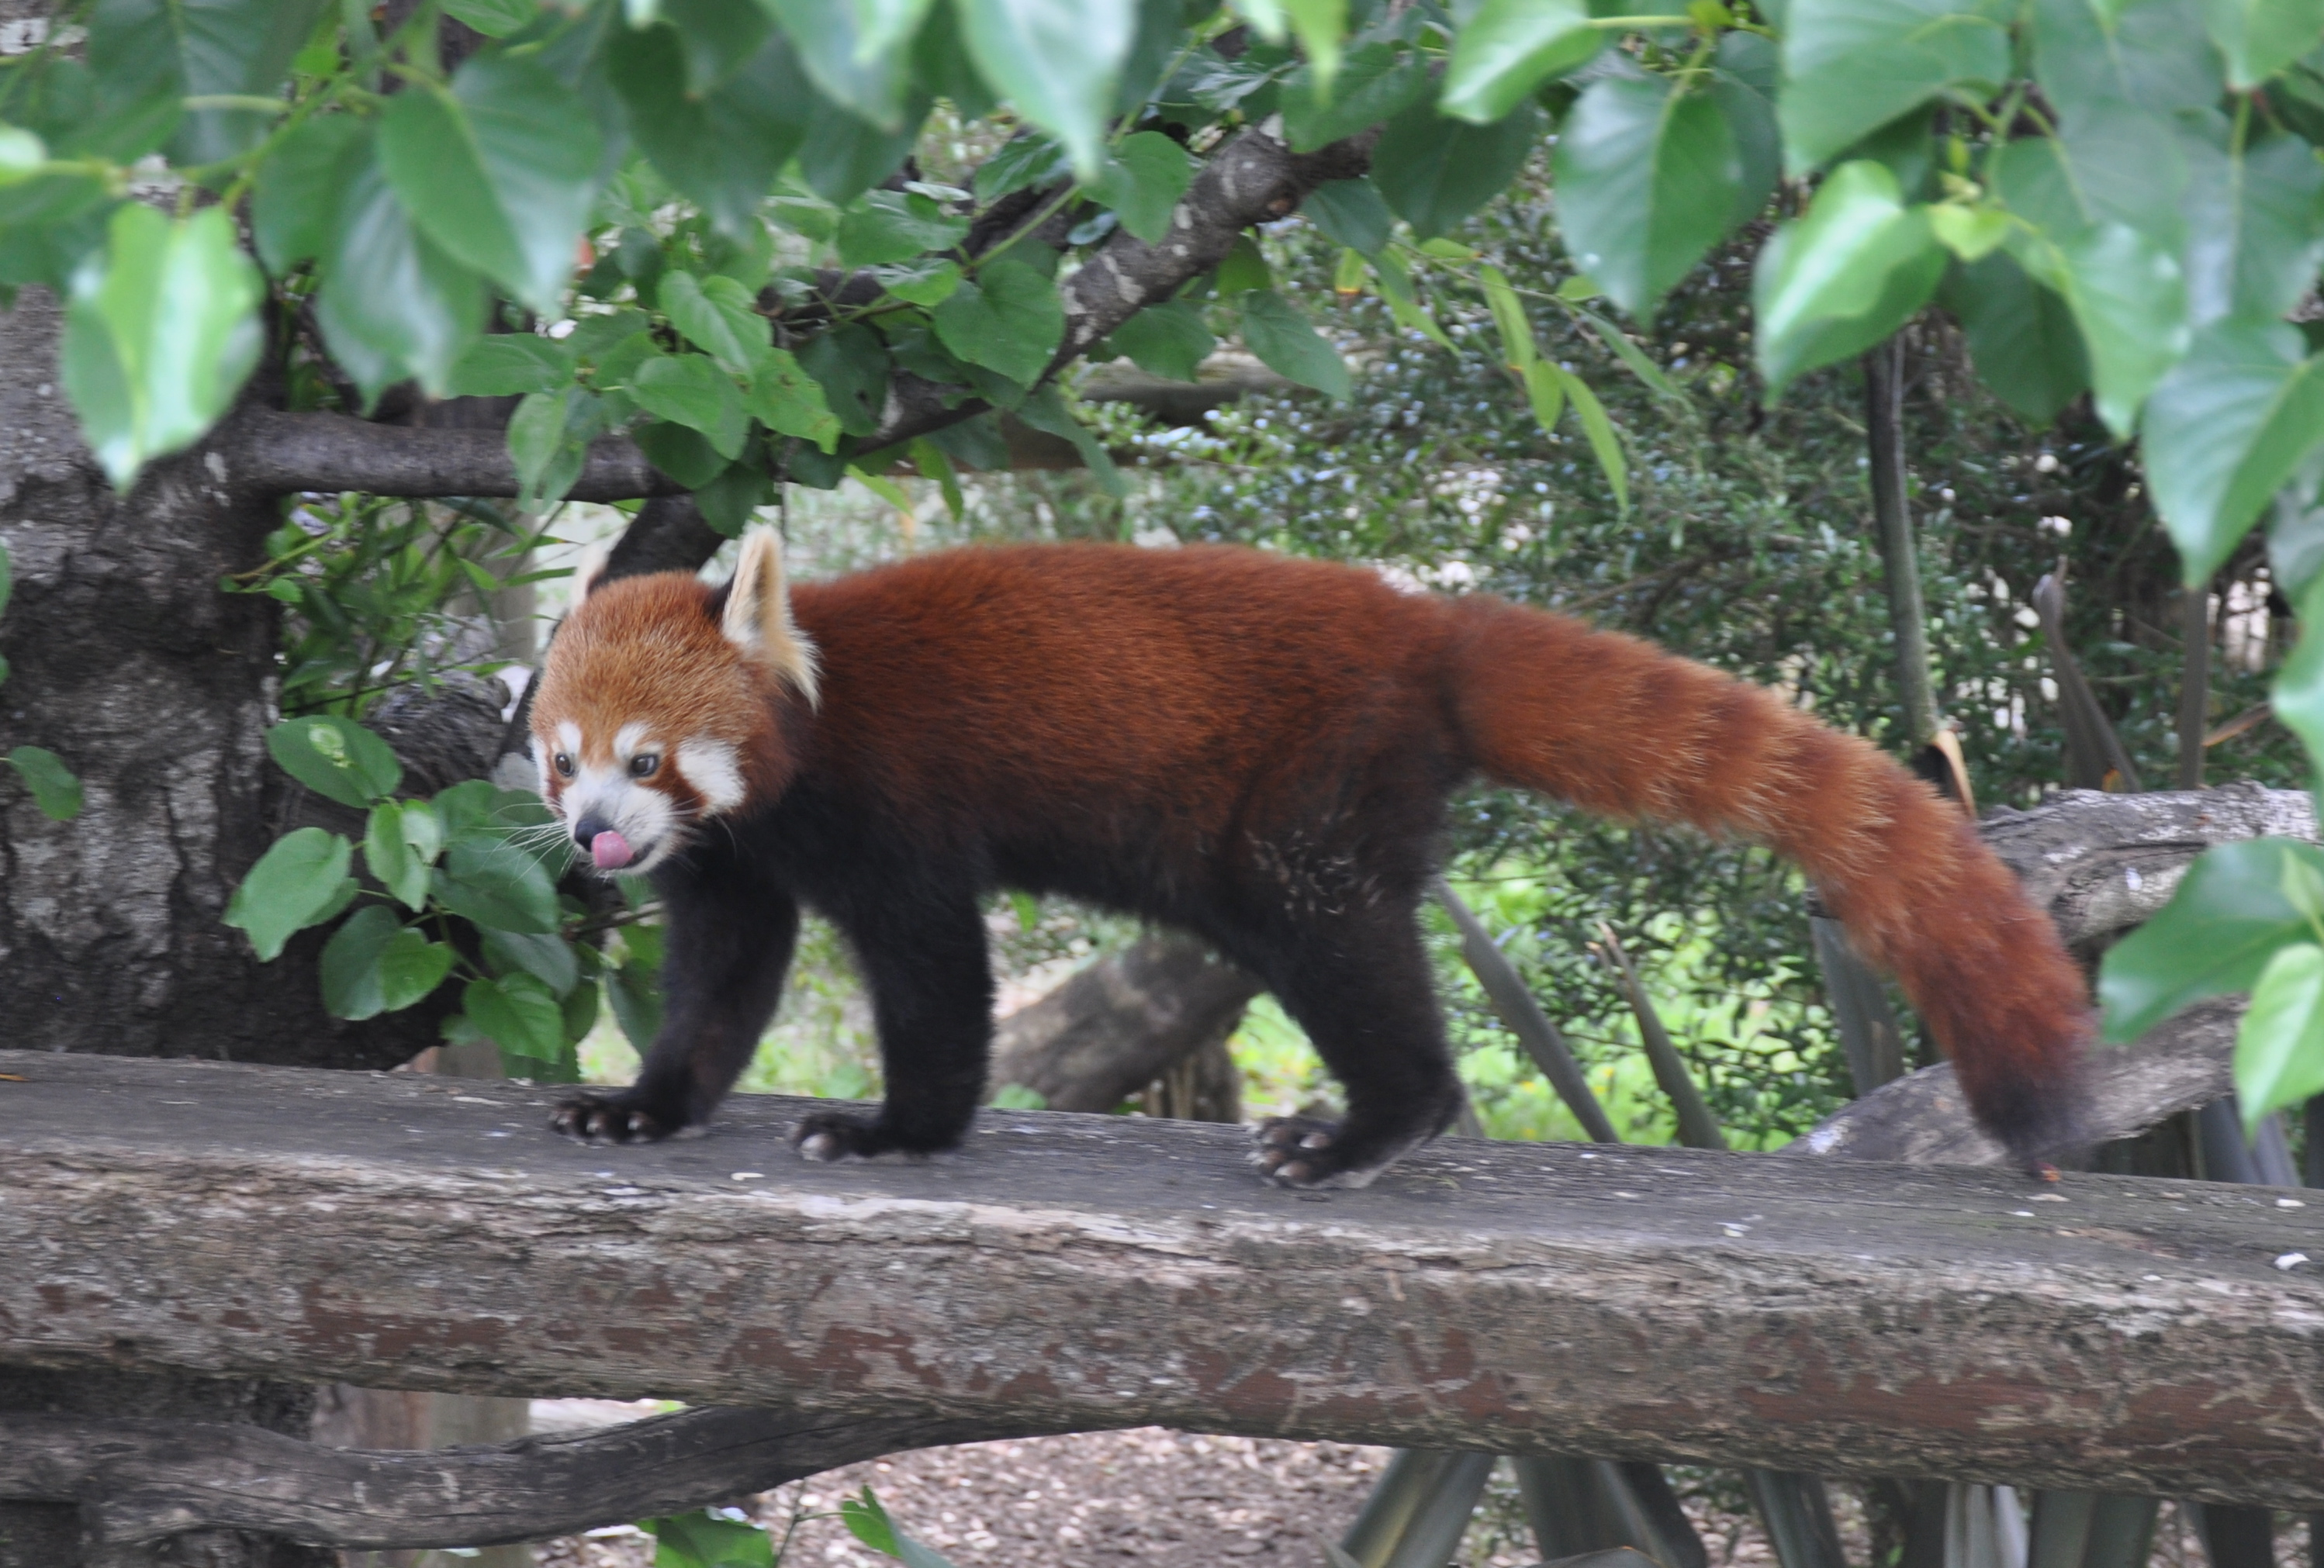
\includegraphics[width = .9 \textwidth]{figures/panda.JPG}
\end{center}
\caption{Le panda roux qui tire la langue. Crew Dragon, ou Dragon 2 (anciennement Dragon V2), est un véhicule spatial développé par la société SpaceX pour le compte de l'agence spatiale américaine, la NASA, pour effectuer la relève des équipages de la Station spatiale internationale. Le vaisseau est capable de transporter un équipage de sept astronautes en orbite basse. Crew Dragon est l'un des deux vaisseaux développés en réponse à l'appel d'offres du programme CCDeV lancé en 2010 ; celui-ci avait pour objectif de reprendre les missions assurées provisoirement par les vaisseaux russes Soyouz à la suite du retrait de la navette spatiale américaine en 2011. }
\label{fig:panda_roux}
\end{figure}

\section{Tables et tableaux}

\section{Tabular}

Du texte \dots \unit{10}\angstrom

\begin{tabular}{cccc}
\hline
\textbf{Nom} & \textbf{Prénom} & \textbf{Age} & Poids \\
\hline
Billson & Bill & $50$ & \unit{10}\pico\newton\per\second\squared\\
%\hline
Truc & Machin & $12$ & \unit{20000}\micro\newton \\
\hline
\end{tabular}

%\blindmathpaper[50]

\section{Modifications de l’environnement }

On voudrait ajouter un espace vertical. \blindtext
\vspace{1cm}

Entre ces deux phrases. \blindtext

\section{Dummy text}
\blindmathpaper[10]

\listoffigures


\end{document}